\subsection{Formatowanie tekstu}

Nasz translator umożliwia pogrubienie, kursywa, podkreślenie, wyśrodkowanie tekstu oraz utworzenie paragrafu. Możliwe jest mieszanie
stylów formatowania, np. pogrubienie z podkreśleniem. Według nowych zaleceń, do pogrubienia tekstu w HTMLu powinno się stosować znacznik
"strong", a do kursywy "em".

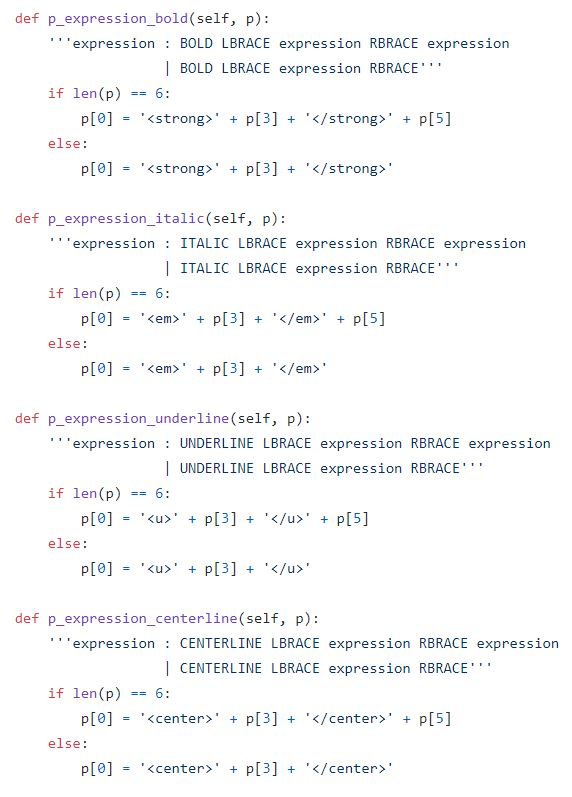
\includegraphics{bold_italic_underline_centerline.JPG}

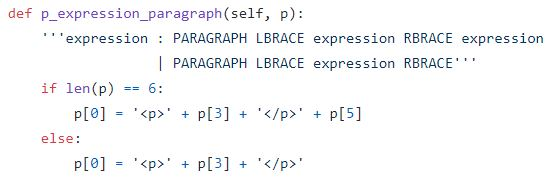
\includegraphics{paragraph.JPG}

Kolejną funkcjonalnością jest możliwość obsługi rozdziałów, sekcji i podsekcji parsując znaczniki chapter, section, subsection, 
subsubsection.


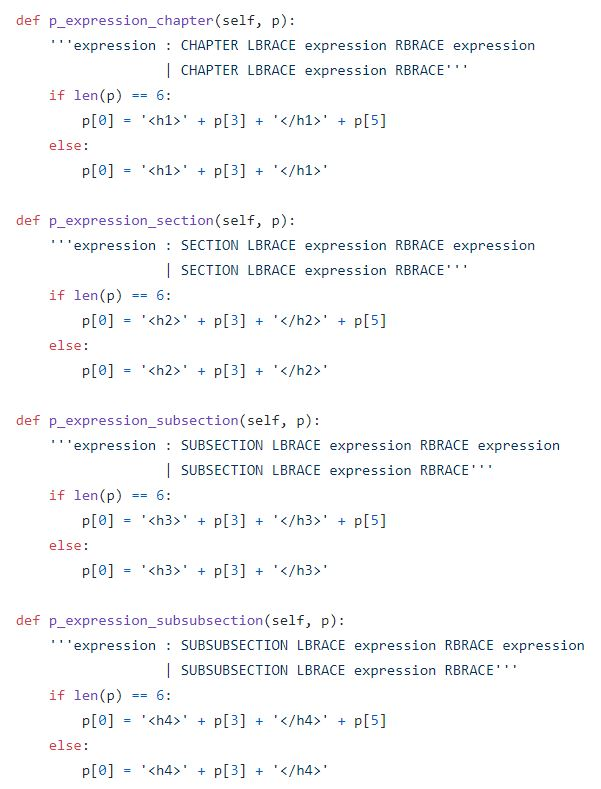
\includegraphics{chapter_section.JPG}


Przejście do nowej linii (hard break) jest obsłużony poleceniem newline.

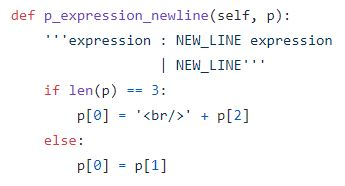
\includegraphics{newline.JPG}


Translator parsuje również znacznik title odpowiadjący z utworzenie tytułu.

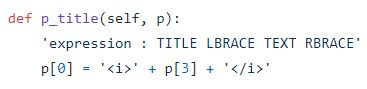
\includegraphics{title.JPG}